
%{{第十六回}}{第十六回}}

\chapter{贾元春才选凤藻宫\hspace{.5em}秦鲸卿夭逝黄泉路}

{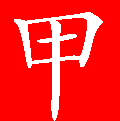
\includegraphics[width=3mm]{../Images/00002}\kaishu 幼儿小女之死,得情之正气,又为痴贪辈一针灸。}

{\kaishu 凤姐恶迹多端,莫大于此件者:受赃婚以致人命。}

{\kaishu 贾府连日闹热非常,宝玉无见无闻,却是宝玉正文。夹写秦、智数句,下半回方不突然。}

{\kaishu 黛玉回,方解宝玉为秦钟之忧闷,是天然之章法。平儿借香菱答话,是补菱姐近来着落。}

{\kaishu 赵妪讨情闲文,却引出通部脉络。所谓由小及大,譬如登高必自卑之意。细思大观园一事,若从如何奉旨起造,又如何分派众人,从头细细直写将来,几千样细事,如何能顺笔一气写清?又将落于死板拮据之乡,故只用琏凤夫妻二人一问一答,上用赵妪讨情作引,下文蓉蔷来说事作收,馀者随笔顺笔略一点染,则耀然洞彻矣。此是避难法。}

{\kaishu 大观园用省亲事出题,是大关键处,方见大手笔行文之立意。}

{\kaishu 借省亲事写南巡,出脱心中多少忆昔感今。}

{\kaishu 极热闹极忙中写秦钟夭逝,可知除“情”字,俱非宝玉正文。}

{\kaishu 大鬼小鬼论势利兴衰,骂尽攒炎附势之辈。}

{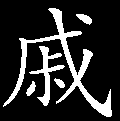
\includegraphics[width=3mm]{../Images/00005}  \kaishu 请看财势与情根,万物难逃造化门。旷典传来空好听,那如知己解温存?}

诗曰:\ldots{}\ldots{}

却说宝玉见收拾了外书房,约定与秦钟读夜书。偏那秦钟秉性最弱,因在郊外受了些风霜,又与智能儿偷期绻缱,未免失于调养,{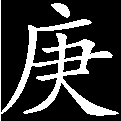
\includegraphics[width=3mm]{../Images/00004}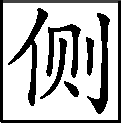
\includegraphics[width=3mm]{../Images/00011}\footnotesize \kaishu 勿笑。这样无能,却是写与人看。}回来时便咳嗽伤风,懒进饮食,大有不胜之态,遂不敢出门,只在家中养息。{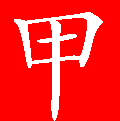
\includegraphics[width=3mm]{../Images/00002}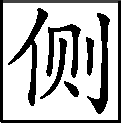
\includegraphics[width=3mm]{../Images/00011}\footnotesize \kaishu 为下文伏线。}宝玉便扫了兴头,只得付于无可奈何,且自静候大愈时再约。{{{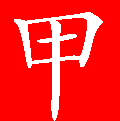
\includegraphics[width=3mm]{../Images/00002}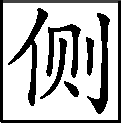
\includegraphics[width=3mm]{../Images/00011}\footnotesize \kaishu 所谓“好事多磨”也。脂砚。}
}\footnote{方括号内的署名表示此署名甲戌本没有但己、庚本有,据补。下同。}

那凤姐儿已是得了云光的回信,俱已妥协。老尼达知张家,果然那守备忍气吞声的收了前聘之物。谁知那个张财主虽如此爱势贪财,却养了一个知义多情的女儿,{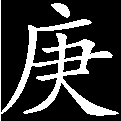
\includegraphics[width=3mm]{../Images/00004}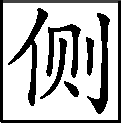
\includegraphics[width=3mm]{../Images/00011}\footnotesize \kaishu 所谓“老鸦窝里出凤凰”,此女是在十二钗之外副者。}闻得父母退了亲事,他便一条绳索悄悄的自缢了。那守备之子闻得金哥自缢,他也是个极多情的,遂也投河而死。{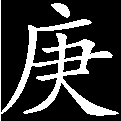
\includegraphics[width=3mm]{../Images/00004}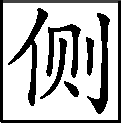
\includegraphics[width=3mm]{../Images/00011}\footnotesize \kaishu 不{[}成{]}双美满夫妻!}只落得张李两家没趣,真是人财两空。这里凤姐却坐享了三千两,{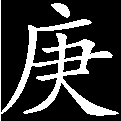
\includegraphics[width=3mm]{../Images/00004}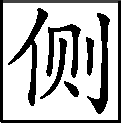
\includegraphics[width=3mm]{../Images/00011}\footnotesize \kaishu 如何消缴?造业者不知,自有知者。}王夫人等连一点消息也不知道。自此凤姐胆识愈壮,以后有了这样的事,便恣意的作为起来,也不消多记。{{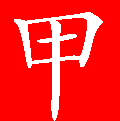
\includegraphics[width=3mm]{../Images/00002}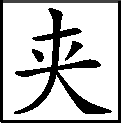
\includegraphics[width=3mm]{../Images/00012}\footnotesize \kaishu 一段收拾过。阿凤心机胆量,真与雨村是一对乱世之奸雄。后文不必细写其事,则知其平生之作为。回首时,无怪乎其惨痛之态,使天下痴心人同来一警,或可期共入于恬然自得之乡矣。脂砚。}

一日,正是贾政的生辰,宁荣二处人丁都齐集庆贺,热闹非常。忽有门吏忙忙进来,至席前报说:“有六宫都太监夏老爷来降旨。”吓得贾赦、贾政等一干人不知是何消息,忙止了戏文,撤去酒席,摆香案启中门跪接。早见六宫都监夏守忠乘马而至,前后左右又有许多内监跟从。那夏守忠也不曾负诏捧敕,至檐前下马,满面笑容,走至厅上,南面而立,口内说:“特旨:立刻宣贾政入朝,在临敬殿陛见。”说毕,也不及吃茶,便乘马去了。贾政等不知是何兆头,只得急忙更衣入朝。{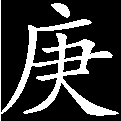
\includegraphics[width=3mm]{../Images/00004}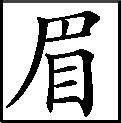
\includegraphics[width=3mm]{../Images/00010}\footnotesize \kaishu 泼天喜事却如此开宗。出人意料外之文也。壬午季春。}

贾母等合家人等心中皆惶惶不定,不住的使人飞马来往报信。有两个时辰工夫,忽见赖大等三四个管家喘吁吁跑进仪门报喜,又说“奉老爷命,速请老太太带领太太等进朝谢恩”等语。那时贾母正心神不定,在大堂廊下伫立,{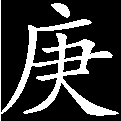
\includegraphics[width=3mm]{../Images/00004}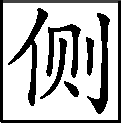
\includegraphics[width=3mm]{../Images/00011}\footnotesize \kaishu 慈母爱子写尽。回廊下伫立,与“日暮倚庐仍怅望”对景,余掩卷而泣。 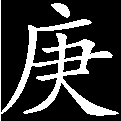
\includegraphics[width=3mm]{../Images/00004}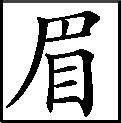
\includegraphics[width=3mm]{../Images/00010}\footnotesize \kaishu “日暮倚庐仍怅望”,南汉先生句也。}邢夫人、王夫人、尤氏、李纨、凤姐、迎春姊妹以及薛姨妈等皆在一处。听如此信至,贾母便唤进赖大来细问端的。赖大禀道:“小的们只在临敬门外伺候,里头的信息一概不能得知。后来还是夏太监出来道喜,说咱家大小姐晋封为凤藻宫尚书,加封贤德妃。后来老爷出来亦如此吩咐小的。如今老爷又往东宫去了,速请老太太领着太太们去谢恩。”贾母等听了方心神安定,不免又都洋洋喜气盈腮。{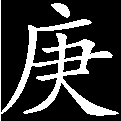
\includegraphics[width=3mm]{../Images/00004}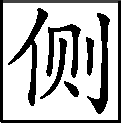
\includegraphics[width=3mm]{../Images/00011}\footnotesize \kaishu 字眼,留神。亦人之常情。}于是都按品大妆起来。贾母带领邢夫人、王夫人、尤氏,一共四乘大轿入朝。贾赦、贾珍亦换了朝服,带领贾蓉、贾蔷奉侍贾母大轿前往。于是宁荣二处上下里外,莫不欣然踊跃,{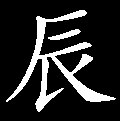
\includegraphics[width=3mm]{../Images/00009}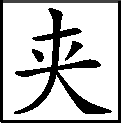
\includegraphics[width=3mm]{../Images/00012}\footnotesize \kaishu 秦氏生魂先告凤姐矣。}个个面上皆有得意之状,言笑鼎沸不绝。

谁知近日水月庵的智能私逃进城,{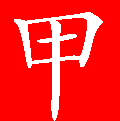
\includegraphics[width=3mm]{../Images/00002}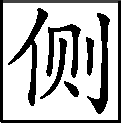
\includegraphics[width=3mm]{../Images/00011}\footnotesize \kaishu 好笔仗,好机轴。 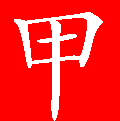
\includegraphics[width=3mm]{../Images/00002}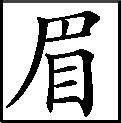
\includegraphics[width=3mm]{../Images/00010}\footnotesize \kaishu 忽然接水月庵,似大脱泄。及读至后,方知为紧收。此大段有如歌急调迫之际,忽闻戛然檀板截断,真见其大力量处,却便于写宝玉之文。}找至秦钟家下看视秦钟,不意被秦业知觉,将智能逐出,将秦钟打了一顿,自己气的老病发作,三五日的光景呜呼死了。秦钟本自怯弱,又值带病未愈,受了笞打,今见老父气死,此时悔痛无及,更又添了许多症候。因此宝玉心中怅然如有所失。{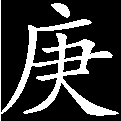
\includegraphics[width=3mm]{../Images/00004}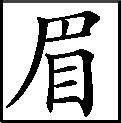
\includegraphics[width=3mm]{../Images/00010}\footnotesize \kaishu 凡用宝玉收拾,俱是大关键。}虽闻得元春晋封之事,亦未解得愁闷。{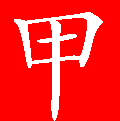
\includegraphics[width=3mm]{../Images/00002}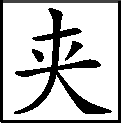
\includegraphics[width=3mm]{../Images/00012}\footnotesize \kaishu 眼前多少{[}热闹{]}文字不写,却从万人意外撰出一段悲伤,是别人不屑写者,亦别人之不能处。}贾母等如何谢恩,如何回家,亲朋如何来庆贺,宁荣两处近日如何热闹,众人如何得意,独他一个皆视有如无,毫不曾介意。{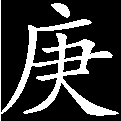
\includegraphics[width=3mm]{../Images/00004}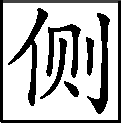
\includegraphics[width=3mm]{../Images/00011}\footnotesize \kaishu 的的真真宝玉。}因此众人嘲他越发呆了。{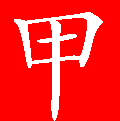
\includegraphics[width=3mm]{../Images/00002}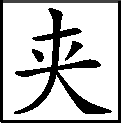
\includegraphics[width=3mm]{../Images/00012}\footnotesize \kaishu 大奇至妙之文,却用宝玉一人,连用五“如何”,隐过多少繁华势利等文。试思若不如此,必至种种写到,其死板拮据、琐碎杂乱,何可胜哉?故只借宝玉一人如此一写,省却多少闲文,却有无限烟波。 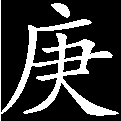
\includegraphics[width=3mm]{../Images/00004}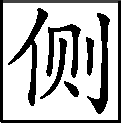
\includegraphics[width=3mm]{../Images/00011}\footnotesize \kaishu 益发呆了。}

且喜贾琏与黛玉回来,先遣人来报信,明日就可到家,宝玉听了,方略有些喜意。{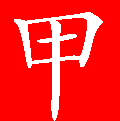
\includegraphics[width=3mm]{../Images/00002}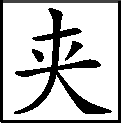
\includegraphics[width=3mm]{../Images/00012}\footnotesize \kaishu 不如此,后文秦钟死去,将何以慰宝玉?}细问原由,方知贾雨村也进京陛见,皆由王子腾累上保本,此来候补京缺,与贾琏是同宗弟兄,又与黛玉有师徒之谊,故同路作伴而来。林如海已葬入祖坟了,诸事停妥,贾琏方进京的。本该出月到家,因闻得元春喜信,遂昼夜兼程而进,一路俱各平安。宝玉只问得黛玉“平安”二字,馀者也就不在意了。{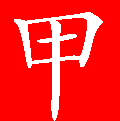
\includegraphics[width=3mm]{../Images/00002}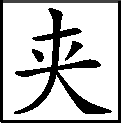
\includegraphics[width=3mm]{../Images/00012}\footnotesize \kaishu 又从天外写出一段离合来,总为掩过宁、荣两处许多琐细闲笔。处处交代清楚,方好起大观园也。}

好容易{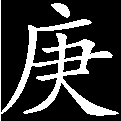
\includegraphics[width=3mm]{../Images/00004}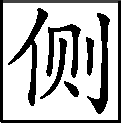
\includegraphics[width=3mm]{../Images/00011}\footnotesize \kaishu 三字是宝玉心中。}盼至明日午错,果报:“琏二爷和林姑娘进府了。”见面时彼此悲喜交接,未免又大哭一阵,后又致喜庆之词。{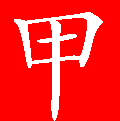
\includegraphics[width=3mm]{../Images/00002}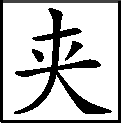
\includegraphics[width=3mm]{../Images/00012}\footnotesize \kaishu 世界上亦如此,不独书中瞬息。观此便可省悟。}宝玉心中品度黛玉,越发出落的超逸了。黛玉又带了许多书籍来,忙着打扫卧室,安插器具,又将些纸笔等物分送宝钗、迎春、宝玉等人。宝玉又将北静王所赠鹡鸰香串珍重取出来,转赠黛玉。黛玉说:“什么臭男人拿过的!我不要他。”遂掷而不取。宝玉只得收回,暂且无话。{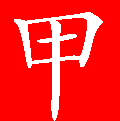
\includegraphics[width=3mm]{../Images/00002}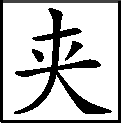
\includegraphics[width=3mm]{../Images/00012}\footnotesize \kaishu 略一点黛玉性情,赶忙收住,正留为后文地步。}

且说贾琏自回家参见过众人,回至房中。正值凤姐近日多事之时,无片刻闲暇之工,{\includegraphics[width=3mm]{../Images/00002}\includegraphics[width=3mm]{../Images/00012}\footnotesize \kaishu 补阿凤二句,最不可少。}见贾琏远路归来,少不得拨冗接待,{\includegraphics[width=3mm]{../Images/00004}\includegraphics[width=3mm]{../Images/00011}\footnotesize \kaishu 写得尖利刻薄。}房内无外人,便笑道:“国舅老爷大喜!国舅老爷一路风尘辛苦。{\includegraphics[width=3mm]{../Images/00002}\includegraphics[width=3mm]{../Images/00011}\footnotesize \kaishu 娇音如闻,俏态如见,少年夫妻常事,的确有之。}小的听见昨日的头起报马来报,说今日大驾归府,略预备了一杯水酒掸尘,{\includegraphics[width=3mm]{../Images/00004}\includegraphics[width=3mm]{../Images/00011}\footnotesize \kaishu 却是为下文作引。}不知可赐光谬领否?”贾琏笑道:“岂敢岂敢,多承多承!”{\includegraphics[width=3mm]{../Images/00004}\includegraphics[width=3mm]{../Images/00011}\footnotesize \kaishu 一言答不上,蠢才蠢才!}一面平儿与众丫鬟参拜毕,献茶。贾琏遂问别后家中的事,又谢凤姐操持劳碌。凤姐道:“我那里照管得这些事!见识又浅,口角又夯,心肠又直率,人家给个棒槌,我就认作针。脸又软,搁不住人给两句好话,心里就慈悲了。况且又无经历过大事,胆子又小,太太略有些不自在,就吓得我连觉也睡不着了。我苦辞了几回,太太又不容辞,倒反说我图受用了,不肯习学了。殊不知我是捻着一把汗儿呢。一句也不敢多说,一步也不敢多走。{\includegraphics[width=3mm]{../Images/00002}\includegraphics[width=3mm]{../Images/00010}\footnotesize \kaishu 此等文字,作者尽力写来,欲诸公认识阿凤,好看后文,勿为泛泛看过。}你是知道的,咱们家所有的这些管家奶奶们,那一位是好缠的?{{\includegraphics[width=3mm]{../Images/00002}\includegraphics[width=3mm]{../Images/00011}\footnotesize \kaishu 独这一句不假。脂砚。}错一点儿他们就笑话打趣,偏一点儿他们就指桑说槐的抱怨。‘坐山观虎’、‘借剑杀人’、‘引风吹火’、‘站干岸儿’、‘推倒油瓶不扶’,都是全挂子的武艺。况且我年纪轻,头等不压众,怨不得不放我在眼里。更可笑{\includegraphics[width=3mm]{../Images/00004}\includegraphics[width=3mm]{../Images/00011}\footnotesize \kaishu 三字是得意口气。}那府里忽然蓉儿媳妇死了,珍大哥又再三再四的在太太跟前跪着讨情,只要请我帮他几日;我是再四推辞,太太断不依,只得从命。依旧被我闹了个马仰人翻,{\includegraphics[width=3mm]{../Images/00004}\includegraphics[width=3mm]{../Images/00011}\footnotesize \kaishu 得意之至口气。}更不成个体统,至今珍大哥还抱怨后悔呢。你这一来了,明儿你见了他,好歹描补描补,就说我年纪小,原没见过世面,谁叫大爷错委他的。”{\includegraphics[width=3mm]{../Images/00002}\includegraphics[width=3mm]{../Images/00010}\footnotesize \kaishu 阿凤之待琏兄如弄小儿,可畏之至。 \includegraphics[width=3mm]{../Images/00004}\includegraphics[width=3mm]{../Images/00011}\footnotesize \kaishu 阿凤之弄琏兄如弄小儿,可怕可畏!若生于小户,落在贫家,琏兄死矣!}

正说着,{\includegraphics[width=3mm]{../Images/00002}\includegraphics[width=3mm]{../Images/00012}\footnotesize \kaishu 又用断法方妙。盖此等文断不可无,亦不可太多。}只听外间有人说话,凤姐便问:“是谁?”平儿进来回道:“姨太太打发香菱妹子来问我一句话,我已经说了,打发他回去了。”贾琏笑道:“正是呢,方才我见姨妈去,不防和一个年轻的小媳妇子撞了个对面,生的好齐整模样。{\includegraphics[width=3mm]{../Images/00004}\includegraphics[width=3mm]{../Images/00011}\footnotesize \kaishu 酒色之徒。}我疑惑咱家并无此人,说话时因问姨妈,谁知就是上京来买的那小丫头,名叫香菱的,竟与薛大傻子作了房里人,开了脸,越发出挑的标致了。那薛大傻子真玷辱了他。”{{\includegraphics[width=3mm]{../Images/00002}\includegraphics[width=3mm]{../Images/00012}\footnotesize \kaishu 垂涎如见。试问兄,宁不有玷平儿乎?脂砚。}凤姐道:“嗳!{\includegraphics[width=3mm]{../Images/00004}\includegraphics[width=3mm]{../Images/00011}\footnotesize \kaishu 如闻。}往苏杭走了一趟回来,也该见些世面了,{\includegraphics[width=3mm]{../Images/00002}\includegraphics[width=3mm]{../Images/00011}\footnotesize \kaishu 这“世面”二字,单指女色也。}还是这么眼馋肚饱的。你要爱他,不值什么,我去拿平儿换了他来如何?{\includegraphics[width=3mm]{../Images/00002}\includegraphics[width=3mm]{../Images/00012}\footnotesize \kaishu 奇谈,是阿凤口中方有此等语句。 \includegraphics[width=3mm]{../Images/00002}\includegraphics[width=3mm]{../Images/00010}\footnotesize \kaishu 用平儿口头谎言,写补菱卿一项实事,并无一丝痕迹,而作者有多少机括。}那薛老大{\includegraphics[width=3mm]{../Images/00002}\includegraphics[width=3mm]{../Images/00011}\footnotesize \kaishu 又一样称呼,各得神理。}也是‘吃着碗里望着锅里’的,这一年来的光景,他为要香菱不能到手,{{\includegraphics[width=3mm]{../Images/00002}\includegraphics[width=3mm]{../Images/00011}\footnotesize \kaishu 补前文之未到,且并将香菱身分写出。脂砚。}和姨妈打了多少饥荒。也因姨妈看着香菱的模样儿好还是末则,其为人行事,却又比别的女孩儿不同,温柔安静,差不多的主子姑娘也跟他不上呢,{\includegraphics[width=3mm]{../Images/00002}\includegraphics[width=3mm]{../Images/00012}\footnotesize \kaishu 何曾不是主子姑娘?盖卿不知来历也。作者必用阿凤一赞,方知莲卿尊重不虚。}故此摆酒请客的费事,明堂正道的与他作了妾。过了没半月,也看的马棚风一般了,我倒心里可惜了的。”{\includegraphics[width=3mm]{../Images/00002}\includegraphics[width=3mm]{../Images/00012}\footnotesize \kaishu 一段纳宠之文,偏于阿凤口中补出,亦奸猾幻妙之至!}一语未了,二门上小厮传报:“老爷在大书房等二爷呢。”贾琏听了,忙忙整衣出去。

这里凤姐乃问平儿:“方才姨妈有什么事,巴巴的打发香菱来?”{\includegraphics[width=3mm]{../Images/00002}\includegraphics[width=3mm]{../Images/00011}\footnotesize \kaishu 必有此一问。}平儿笑道:“那里来的香菱,是我借他暂撒个谎。{\includegraphics[width=3mm]{../Images/00002}\includegraphics[width=3mm]{../Images/00011}\footnotesize \kaishu 卿何尝谎言?的是补菱姐正文。}奶奶说说,旺儿嫂子越发连个承算也没了。”{\includegraphics[width=3mm]{../Images/00009}\includegraphics[width=3mm]{../Images/00012}\footnotesize \kaishu 此处系平儿捣鬼。}说着,又走至凤姐身边,悄悄说道:{\includegraphics[width=3mm]{../Images/00004}\includegraphics[width=3mm]{../Images/00011}\footnotesize \kaishu 如闻如见。}“奶奶的那利钱银子,迟不送来,早不送来,这会子二爷在家,他且送这个来了。{\includegraphics[width=3mm]{../Images/00002}\includegraphics[width=3mm]{../Images/00011}\footnotesize \kaishu 总是补遗。}幸亏我在堂屋里撞见,不然时走了来回奶奶,二爷倘或问奶奶是什么利钱,奶奶自然不肯瞒二爷的,{\includegraphics[width=3mm]{../Images/00002}\includegraphics[width=3mm]{../Images/00011}\footnotesize \kaishu 平姐欺看书人了。 \includegraphics[width=3mm]{../Images/00004}\includegraphics[width=3mm]{../Images/00011}\footnotesize \kaishu 可儿可儿,凤姐竟被他哄了。}少不得照实告诉二爷。我们二爷那脾气,油锅里的钱还要找出来花呢,听见奶奶有了这个梯己,他还不放心的花了呢?所以我赶着接了过来,叫我说了他两句。谁知奶奶偏听见了问,我就撒谎说香菱了。”{\includegraphics[width=3mm]{../Images/00002}\includegraphics[width=3mm]{../Images/00012}\footnotesize \kaishu 一段平儿的见识作用,不枉阿凤生平刮目,又伏下多少后文,补尽前文未到。}凤姐听了笑道:“我说呢,姨妈知道你二爷来了,忽喇八的反打发个房里人来了?原来你这蹄子肏鬼。”{\includegraphics[width=3mm]{../Images/00004}\includegraphics[width=3mm]{../Images/00011}\footnotesize \kaishu 疼极反骂。}

说话时,贾琏已进来,凤姐便命摆上酒馔来,夫妻对坐。凤姐虽善饮,却不敢任兴,{\includegraphics[width=3mm]{../Images/00002}\includegraphics[width=3mm]{../Images/00012}\footnotesize \kaishu 百忙中又点出大家规范,所谓无不周详,无不贴切。}只陪着贾琏。一时贾琏的乳母赵嬷嬷走来,贾琏与凤姐忙让他一同吃酒,令其上炕去。赵嬷嬷执意不肯。平儿等早已炕沿下设下一杌子,又有一小脚踏,赵嬷嬷在脚踏上坐了。贾琏向桌上拣两盘肴馔,与他放在杌上自吃。凤姐又道:“妈妈很咬不动那个,倒没的硌了他的牙。”{\includegraphics[width=3mm]{../Images/00004}\includegraphics[width=3mm]{../Images/00011}\footnotesize \kaishu 何处着想,却是自然有的。}因向平儿道:“早起我说那一碗火腿炖肘子很烂,正好给妈妈吃,你怎么不取去赶着叫他们热来?”又道:“妈妈,你尝一尝你儿子带来的惠泉酒。”{\includegraphics[width=3mm]{../Images/00004}\includegraphics[width=3mm]{../Images/00011}\footnotesize \kaishu 补点不到之文,像极!}赵嬷嬷道:“我喝呢,奶奶也喝一钟。怕什么,只不要过多了就是了。{\includegraphics[width=3mm]{../Images/00002}\includegraphics[width=3mm]{../Images/00012}\footnotesize \kaishu 宝玉之李嬷,此处偏又写一赵嬷,特犯不犯。先有梨香院一回,今又写此一回,两两遥对,却无一笔相重,一事合掌。}我这会子跑来,倒也不为酒饭,倒有一件正经事,奶奶好歹记在心里,疼顾我些罢。我们的爷,只是嘴里说的好,到了跟前就忘了我们。幸亏我从小儿奶了你这么大。我也老了,有的是那两个儿子,你就另眼照看他们些,别人也不敢呲牙儿的。{\includegraphics[width=3mm]{../Images/00004}\includegraphics[width=3mm]{../Images/00011}\footnotesize \kaishu 为蔷、蓉作引。}我还再四的求了你几遍,你答应的倒好,到如今还是燥屎。{\includegraphics[width=3mm]{../Images/00004}\includegraphics[width=3mm]{../Images/00011}\footnotesize \kaishu 有是乎?}这如今又从天上跑出这样一件大喜事来,那里用不着人?所以倒是来求奶奶是正经。靠着我们爷,只怕我还饿死了呢。”

凤姐笑道:“妈妈你放心,两个奶哥哥都交给我。你从小儿奶的,你还有什么不知道他那脾气的?拿着皮肉倒往那不相干的外人身上贴。可是现放着奶哥哥,那一个不比人强?你疼顾照看他们,谁敢说个‘不’字儿?{\includegraphics[width=3mm]{../Images/00004}\includegraphics[width=3mm]{../Images/00011}\footnotesize \kaishu 会送情。}没的白便宜了外人。------我这话也说错了,我们看着是‘外人’,你却是看着是‘内人’一样呢。”{\includegraphics[width=3mm]{../Images/00004}\includegraphics[width=3mm]{../Images/00011}\footnotesize \kaishu 可儿可儿!}说的满屋里人都笑了。赵嬷嬷也笑个不住,又念佛道:“可是屋子里跑出青天来了!若说‘内人’‘外人’这些混帐事,我们爷是没有,{\includegraphics[width=3mm]{../Images/00002}\includegraphics[width=3mm]{../Images/00011}\footnotesize \kaishu 千真万真,是没有。一笑。 \includegraphics[width=3mm]{../Images/00004}\includegraphics[width=3mm]{../Images/00011}\footnotesize \kaishu 有是语,像极,毕肖。乳母护子。}不过是脸软心慈,搁不住人求两句罢了。”凤姐笑道:“可不是呢,有‘内人’求的他才慈软呢,他在咱们娘儿们跟前才是刚硬呢!”赵嬷嬷笑道:“奶奶说的太尽情了,我也乐了。再吃一杯好酒。从此我们奶奶作了主,我就没的愁了。”

贾琏此时没好意思,只是讪笑吃酒,说“胡说”二字,“快盛饭来,吃碗子还要往珍大爷那边去商议事呢。”凤姐道:“可是。别误了正事。才刚老爷叫你说什么?”{\includegraphics[width=3mm]{../Images/00003}\includegraphics[width=3mm]{../Images/00012}\footnotesize \kaishu 一段赵妪讨情闲文,却引出通部脉络。所谓由小及大,譬如登高必自卑之意。细思大观园一事,若从如何奉旨起造,又如何分派众人,从头细细直写将来,几千样细事,如何能顺笔一气写清?又将落于死板拮据之乡,故只用琏凤夫妻二人一问一答,上用赵妪讨情作引,下用蓉蔷来说事作收,馀者随笔顺笔略一点染,则耀然洞彻矣。此是避难法。}贾琏道:“就为省亲。”{\includegraphics[width=3mm]{../Images/00002}\includegraphics[width=3mm]{../Images/00012}\footnotesize \kaishu 二字醒眼之极,却只如此写来。 \includegraphics[width=3mm]{../Images/00004}\includegraphics[width=3mm]{../Images/00010}\footnotesize \kaishu 大观园用省亲事出题,是大关键事,方见大手笔行文之立意。畸笏。}凤姐忙问道:{\includegraphics[width=3mm]{../Images/00002}\includegraphics[width=3mm]{../Images/00012}\footnotesize \kaishu “忙”字最要紧,特于凤姐口中出此字,可知事关巨要,非同浅细,是此书中正眼矣。}“省亲的事竟准了不成?”{{\includegraphics[width=3mm]{../Images/00002}\includegraphics[width=3mm]{../Images/00012}\footnotesize \kaishu 问得珍重,可知是万人意外之事。脂砚。}贾琏笑道:“虽不十分准,也有八分准了。”{\includegraphics[width=3mm]{../Images/00002}\includegraphics[width=3mm]{../Images/00012}\footnotesize \kaishu 如此故顿一笔,更妙!见得事关重大,非一语可了者,亦是大篇文章,抑扬顿挫之至。}凤姐笑道:“可见当今的隆恩。历来听书看戏,古时从来未有的。”{{\includegraphics[width=3mm]{../Images/00002}\includegraphics[width=3mm]{../Images/00012}\footnotesize \kaishu 于闺阁中作此语,直与《击壤》同声。脂砚。}赵嬷嬷又接口道:“可是呢,我也老糊涂了。我听见上上下下吵嚷了这些日子,什么省亲不省亲,我也不理论他去;如今又说省亲,到底是怎么个原故?”{\includegraphics[width=3mm]{../Images/00002}\includegraphics[width=3mm]{../Images/00011}\footnotesize \kaishu 补近日之事,启下回之文。 \includegraphics[width=3mm]{../Images/00002}\includegraphics[width=3mm]{../Images/00010}\footnotesize \kaishu 赵嬷一问,是文章家进一步门庭法则。 \includegraphics[width=3mm]{../Images/00004}\includegraphics[width=3mm]{../Images/00010}\footnotesize \kaishu 自政老生日,用降旨截住,贾母等进朝如此热闹,用秦业死岔开,只写几个“如何”,将泼天喜事交代完了。紧接黛玉回,琏、凤闲话,以老妪勾出省亲事来。其千头万绪,合榫贯连,无一毫痕迹,如此等,是书多多,不能枚举。想兄在青埂峰上,经煅炼后,参透重关至恒河沙数。如否,余曰万不能有此机括,有此笔力,恨不得面问果否。叹叹!丁亥春。畸笏叟。}贾琏道:{\includegraphics[width=3mm]{../Images/00002}\includegraphics[width=3mm]{../Images/00011}\footnotesize \kaishu 大观园一篇大文,千头万绪,从何处写起?今故用贾琏夫妻问答之间,闲闲叙出,观者已省大半。后再用蓉、蔷二人重一渲染。便省却多少赘瘤笔墨。此是避难法。}“如今当今体贴万人之心,世上至大莫如‘孝’字,想来父母儿女之性,皆是一理,不是贵贱上分别的。当今自为日夜侍奉太上皇、皇太后,尚不能略尽孝意,因见宫里嫔妃、才人等皆是入宫多年,以致抛离父母音容,岂有不思想之理?在儿女,思想父母是分所应当。想父母在家,若只管思念儿女,竟不能一见,倘因此成疾致病,甚至死亡,皆由朕躬禁锢,不能使其遂天伦之愿,亦大伤天和之事。故启奏太上皇、皇太后,每月逢二六日期,准其椒房眷属入宫请候看视。于是太上皇、皇太后大喜,深赞当今至孝纯仁,体天格物。因此二位老圣人又下旨意,说椒房眷属入宫,未免有国体仪制,母女尚不能惬怀。竟大开方便之恩,特降谕诸椒房贵戚,除二六日入宫之恩外,凡有重宇别院之家,可以驻跸关防之处,不妨启请内廷銮舆入其私第,庶可略尽骨肉私情、天伦中之至性。此旨一下,谁不踊跃感戴?现今周贵人的父亲已在家里动了工了,修盖省亲别院呢。又有吴贵妃的父亲吴天佑家,也往城外踏看地方去了。{\includegraphics[width=3mm]{../Images/00002}\includegraphics[width=3mm]{../Images/00011}\footnotesize \kaishu 又一样布置。}这岂不有八九分了?”

赵嬷嬷道:“阿弥陀佛!原来如此。这样说,咱们家也要预备接咱们大小姐了?”{\includegraphics[width=3mm]{../Images/00004}\includegraphics[width=3mm]{../Images/00011}\footnotesize \kaishu 文忠公之嬷。}贾琏道:“这何用说呢!不然,这会子忙的是什么?”{\includegraphics[width=3mm]{../Images/00002}\includegraphics[width=3mm]{../Images/00011}\footnotesize \kaishu 一段闲谈中补出多少文章。真是费长房“壶中天地”也。}凤姐笑道:“若果如此,我可也见个大世面了。可恨我小几岁年纪,若早生二三十年,如今这些老人家也不薄我没见世面了。{\includegraphics[width=3mm]{../Images/00002}\includegraphics[width=3mm]{../Images/00011}\footnotesize \kaishu 忽接入此句,不知何意?似属无谓。}说起当年太祖皇帝仿舜巡的故事,比一部书还热闹,{\includegraphics[width=3mm]{../Images/00004}\includegraphics[width=3mm]{../Images/00011}\footnotesize \kaishu 既知舜巡而又说热闹,此妇人女子口头也。}我偏没造化赶上。”{\includegraphics[width=3mm]{../Images/00004}\includegraphics[width=3mm]{../Images/00011}\footnotesize \kaishu 不用忙,往后看。}赵嬷嬷道:“嗳哟哟,那可是千载希逢的!那时候我才记事儿,咱们贾府正在姑苏、扬州一带监造海舫,修理海塘,只预备接驾一次,{\includegraphics[width=3mm]{../Images/00004}\includegraphics[width=3mm]{../Images/00011}\footnotesize \kaishu 又要瞒人。}把银子都花的淌海水似的!说起来\ldots{}\ldots{}”凤姐忙接道:{\includegraphics[width=3mm]{../Images/00002}\includegraphics[width=3mm]{../Images/00011}\footnotesize \kaishu 又截得好。{$\diamond$}“忙”字妙!上文“说起来”必未完,粗心看去则说疑阙,殊不知正传神处。}“我们王府也预备过一次。那时我爷爷单管各国进贡朝贺的事,凡有的外国人来,都是我们家养活。{\includegraphics[width=3mm]{../Images/00002}\includegraphics[width=3mm]{../Images/00011}\footnotesize \kaishu 点出阿凤所有外国奇玩等物。}粤、闽、滇、浙所有的洋船货物,都是我们家的。”

赵嬷嬷道:“那是谁不知道的?如今还有个口号儿呢,说‘东海少了白玉床,龙王来请江南王’,{\includegraphics[width=3mm]{../Images/00004}\includegraphics[width=3mm]{../Images/00011}\footnotesize \kaishu 应前“葫芦案”。}这说的就是奶奶府上了。还有如今现在江南的甄家,{\includegraphics[width=3mm]{../Images/00002}\includegraphics[width=3mm]{../Images/00011}\footnotesize \kaishu 甄家正是大关键、大节目,勿作泛泛口头语看。}嗳哟哟,{\includegraphics[width=3mm]{../Images/00004}\includegraphics[width=3mm]{../Images/00011}\footnotesize \kaishu 口气如闻。}好势派!独他家接驾四次。{\includegraphics[width=3mm]{../Images/00004}\includegraphics[width=3mm]{../Images/00011}\footnotesize \kaishu 点正题正文。}若不是我们亲眼看见,告诉谁谁也不信的。别讲银子成了土泥,{\includegraphics[width=3mm]{../Images/00004}\includegraphics[width=3mm]{../Images/00011}\footnotesize \kaishu 极力一写,非夸也,可想而知。}凭是世上所有的,没有不是堆山塞海的,‘罪过可惜’四个字,竟顾不得了。”{\includegraphics[width=3mm]{../Images/00004}\includegraphics[width=3mm]{../Images/00011}\footnotesize \kaishu 真有是事,经过见过。}凤姐道:“我常听见我们太爷们也这样说,岂有不信的。{\includegraphics[width=3mm]{../Images/00004}\includegraphics[width=3mm]{../Images/00011}\footnotesize \kaishu 对证。}只纳罕他家怎么就这么富贵呢?”赵嬷嬷道:“告诉奶奶一句话,也不过是拿着皇帝家的银子往皇帝身上使罢了!{\includegraphics[width=3mm]{../Images/00002}\includegraphics[width=3mm]{../Images/00011}\footnotesize \kaishu 是不忘本之言。}谁家有那些钱买这个虚热闹去?”{\includegraphics[width=3mm]{../Images/00002}\includegraphics[width=3mm]{../Images/00011}\footnotesize \kaishu 最要紧语。人苦不自知。能作是语者吾未尝见。}

正说的热闹,王夫人又打发人来瞧凤姐吃了饭不曾。凤姐便知有事等他,忙忙的吃了半碗饭,漱口要走,{\includegraphics[width=3mm]{../Images/00004}\includegraphics[width=3mm]{../Images/00011}\footnotesize \kaishu 好顿挫。}又有二门上小厮们回:“东府里蓉、蔷二位哥儿来了。”贾琏才漱了口,平儿捧着盆盥手,见他二人来了,便问:“什么话?快说。”凤姐且止步稍候,听他二人回些什么。贾蓉先回说:“我父亲打发我来回叔叔:老爷们已经议定了,{\includegraphics[width=3mm]{../Images/00004}\includegraphics[width=3mm]{../Images/00011}\footnotesize \kaishu 简净之至!}从东边一带,借着东府里的花园起,转至北边,一共丈量准了,三里半大,可以盖造省亲别院了。{\includegraphics[width=3mm]{../Images/00004}\includegraphics[width=3mm]{../Images/00011}\footnotesize \kaishu 园基乃一部之主,必当如此写清。}已经传人画图样去了,{\includegraphics[width=3mm]{../Images/00004}\includegraphics[width=3mm]{../Images/00011}\footnotesize \kaishu 后一图伏线。大观园系玉兄与十二钗之太虚幻境,岂可草率?}明日就得。叔叔才回家,未免劳乏,不用过我们那边去,{\includegraphics[width=3mm]{../Images/00004}\includegraphics[width=3mm]{../Images/00011}\footnotesize \kaishu 应前贾琏口中。}有话明日一早再请过去面议。”贾琏笑着说道:“多谢大爷费心体谅,我就从命不过去了。正经是这个主意才省事,盖的也容易;若采置别处地方去,那更费事,且倒不成体统。你回去说,这样很好,若老爷们再要改时,全仗大爷谏阻,万不可另寻地方。明日一早我给大爷请安去,再议细话。”贾蓉忙应几个“是”。{\includegraphics[width=3mm]{../Images/00004}\includegraphics[width=3mm]{../Images/00011}\footnotesize \kaishu 园已定矣。}

贾蔷又近前回说:“下姑苏割聘教习,采买女孩子,置办乐器行头等事,大爷派了侄儿,{\includegraphics[width=3mm]{../Images/00004}\includegraphics[width=3mm]{../Images/00011}\footnotesize \kaishu “画蔷”一回伏线。}带领着来管家两个儿子,还有单聘仁、卜固修两个清客相公,一同前往,所以命我来见叔叔。”{\includegraphics[width=3mm]{../Images/00004}\includegraphics[width=3mm]{../Images/00011}\footnotesize \kaishu 凡各物事,工价重大兼伏隐着情字者,莫如此件。故园定后便先写此一件,馀便不必细写矣。}贾琏听了,将贾蔷打量了打量,{\includegraphics[width=3mm]{../Images/00004}\includegraphics[width=3mm]{../Images/00011}\footnotesize \kaishu 有神。}笑道:“你能在这一行么?{\includegraphics[width=3mm]{../Images/00004}\includegraphics[width=3mm]{../Images/00011}\footnotesize \kaishu 勾下文。}这个事虽不甚大,里头大有藏掖的。”{\includegraphics[width=3mm]{../Images/00002}\includegraphics[width=3mm]{../Images/00011}\footnotesize \kaishu 射利人微露心迹。 \includegraphics[width=3mm]{../Images/00004}\includegraphics[width=3mm]{../Images/00011}\footnotesize \kaishu 射利语,可叹!是亲侄。}贾蔷笑道:“只好学习着办罢了。”

贾蓉在身旁灯影下悄拉凤姐的衣襟,凤姐会意,因笑道:“你也太操心了,难道大爷比咱们还不会用人?偏你又怕他不在行了。谁都是在行的?孩子们已长的这么大了,‘没吃过猪肉,也看见过猪跑’。大爷派他去,原不过是个坐纛旗儿,难道认真的叫他去讲价钱、会经纪去呢!依我说就很好。”贾琏道:“自然是这样。并不是我驳回,少不得替他筹算筹算。”因问:“这项银子动那一处的?”贾蔷道:“才也议到这里。赖爷爷{\includegraphics[width=3mm]{../Images/00002}\includegraphics[width=3mm]{../Images/00011}\footnotesize \kaishu 此等称呼,令人酸鼻。 \includegraphics[width=3mm]{../Images/00004}\includegraphics[width=3mm]{../Images/00011}\footnotesize \kaishu 好称呼。}说,竟不用从京里带下去,江南甄家还收着我们五万银子。明日写一封书信,会票我们带去,先支三万,下剩二万存着,等置办花烛彩灯并各色帘栊帐幔的使费。”贾琏点头道:“这个主意好。”{\includegraphics[width=3mm]{../Images/00004}\includegraphics[width=3mm]{../Images/00010}\footnotesize \kaishu 《石头记》中多作心传神会之文,不必道明。一道明白,便入庸俗之套。}

凤姐便向贾蔷道:{{\includegraphics[width=3mm]{../Images/00002}\includegraphics[width=3mm]{../Images/00011}\footnotesize \kaishu 再不略让一步,正是阿凤一生短处。[脂砚。]}}“既这样,我有两个在行妥当人,你就带他们去办,这个便宜了你呢。”贾蔷忙陪笑道:“正要和婶子讨两个人呢,{{\includegraphics[width=3mm]{../Images/00002}\includegraphics[width=3mm]{../Images/00011}\footnotesize \kaishu 写贾蔷乖处。脂砚。}这可巧了。”因问名字。凤姐便问赵嬷嬷。彼时赵嬷嬷已听呆了话,平儿忙笑推他,{\includegraphics[width=3mm]{../Images/00006}\includegraphics[width=3mm]{../Images/00011}\footnotesize \kaishu 真是强将手下无弱兵。至精至细。}他才醒悟过来,忙说:“一个叫赵天梁,一个叫赵天栋。”凤姐道:“可别忘了,我可干我的去了。”说着便出去了。贾蓉忙赶出来,又悄悄向凤姐道:“婶子要带什么东西?”
\footnote{诸本此后有“分付我,开个账给蔷兄弟带了去,叫他按账置办了来。”按贾蓉并非如此罗嗦之人,此处当以底本点到为止较胜。}凤姐笑{\includegraphics[width=3mm]{../Images/00004}\includegraphics[width=3mm]{../Images/00011}\footnotesize \kaishu 有神。}道:“别放你娘的屁!{\includegraphics[width=3mm]{../Images/00004}\includegraphics[width=3mm]{../Images/00011}\footnotesize \kaishu 像极,的是阿凤。}我的东西还没处撂呢,稀罕你们鬼鬼祟祟的?”说着一迳去了。{{\includegraphics[width=3mm]{../Images/00002}\includegraphics[width=3mm]{../Images/00011}\footnotesize \kaishu 阿凤欺人处如此。{$\diamond$}忽又写到利弊,真令人一叹。[脂砚。]{ \includegraphics[width=3mm]{../Images/00004}\includegraphics[width=3mm]{../Images/00010}\footnotesize \kaishu 从头至尾细看阿凤之待蓉、蔷,可谓一体一党,然尚作如此语欺蓉,其待他人可知矣。}}

这里贾蔷也悄问贾琏:“要什么东西?顺便织来孝敬叔叔。”贾琏笑道:“你别兴头。才学着办事,倒先学会这把戏。我短了什么,少不得写信去告诉你,{\includegraphics[width=3mm]{../Images/00004}\includegraphics[width=3mm]{../Images/00011}\footnotesize \kaishu 又作此语,不犯阿凤。}且不要论到这里。”说毕,打发他二人去了。接着回事的人来,不止三四次,贾琏害乏,便传与二门上,一应不许传报,俱等明日料理。凤姐至三更时分方下来安歇,{\includegraphics[width=3mm]{../Images/00004}\includegraphics[width=3mm]{../Images/00011}\footnotesize \kaishu 好文章,一句内隐两处若许事情。}一宿无话。

次日早贾琏起来,见过贾赦、贾政,便往宁府中来,合同老管事人等,并几位世交门下清客相公,审察两府地方,缮画省亲殿宇,一面参度办理人丁。自此后,各行匠役齐集,金银铜锡以及土木砖瓦之物,搬运移送不歇。{\includegraphics[width=3mm]{../Images/00006}\includegraphics[width=3mm]{../Images/00011}\footnotesize \kaishu 一总。}先令匠役拆宁府会芳园墙垣楼阁,直接入荣府东大院中。荣府东边所有下人一带群房尽已拆去。当日宁荣二宅,虽有一小巷界断不通,{\includegraphics[width=3mm]{../Images/00002}\includegraphics[width=3mm]{../Images/00011}\footnotesize \kaishu 补明,使观者如身临足到。}然这小巷亦系私地,并非官道,故可以连属。会芳园本是从北角墙下引来一股活水,今亦无烦再引。{\includegraphics[width=3mm]{../Images/00002}\includegraphics[width=3mm]{../Images/00011}\footnotesize \kaishu 园中诸景,最要紧是水,亦必写明方妙。{$\diamond$}余最鄙近之修造园亭者,徒以顽石土堆为佳,不知引泉一道。甚至丹青,唯知乱作山石树木,不知画泉之法,亦是恨事。{[}脂砚斋。{]}}其山石树木虽不敷用,贾赦住的乃是荣府旧园,其中竹树山石以及亭榭栏杆等物,皆可挪就前来。如此两处又甚近,凑来一处,省得许多财力,纵亦不敷,所添亦有限。全亏一个老明公号山子野{\includegraphics[width=3mm]{../Images/00002}\includegraphics[width=3mm]{../Images/00011}\footnotesize \kaishu 妙号,随事生名。}者,一一筹画起造。

贾政不惯于俗务,{\includegraphics[width=3mm]{../Images/00004}\includegraphics[width=3mm]{../Images/00011}\footnotesize \kaishu 这也少不得的一节文字,省下笔来好作别样。}只凭贾赦、贾珍、贾琏、赖大、来升、林之孝、吴新登、詹光、程日兴等几人安插摆布。凡堆山凿池、起楼竖阁、种竹栽花一应点景等事,又有山子野制度。下朝闲暇,不过各处看望看望,最要紧处和贾赦商议商议便罢了。贾赦只在家高卧,有芥豆之事,贾珍等或自去回明,或写略节;或有话说,便传呼贾琏、赖大等来领命。贾蓉单管打造金银器皿。{\includegraphics[width=3mm]{../Images/00006}\includegraphics[width=3mm]{../Images/00011}\footnotesize \kaishu 好差。}贾蔷已起身往姑苏去了。贾珍、赖大等又点人丁,开册籍,监工等事,一笔不能写到,不过是喧阗热闹非常而已。暂且无话。

且说宝玉近因家中有这等大事,贾政不来问他的书,{\includegraphics[width=3mm]{../Images/00004}\includegraphics[width=3mm]{../Images/00011}\footnotesize \kaishu 一笔不漏。}心中是件畅事。无奈秦钟之病一日重似一日,也着实悬心,不能乐业。{\includegraphics[width=3mm]{../Images/00002}\includegraphics[width=3mm]{../Images/00011}\footnotesize \kaishu “天下本无事,庸人自扰之”,世上人各各如此,又非此情钟意切。 \includegraphics[width=3mm]{../Images/00002}\includegraphics[width=3mm]{../Images/00010}\footnotesize \kaishu 偏于大热闹处写出大不得意之文,却无丝毫牵强,且有许多令人笑不了、哭不了、叹不了、悔不了,惟以大白酬我作者。{[}壬午季春。畸笏。{]}}这日一早起来,才梳洗毕,意欲回了贾母去望候秦钟,忽见茗烟在二门照壁前探头缩脑,宝玉忙出来问他:“作什么?”茗烟道:“秦相公不中用了!”{\includegraphics[width=3mm]{../Images/00002}\includegraphics[width=3mm]{../Images/00011}\footnotesize \kaishu 从茗烟口中写出,省却多少闲文。}宝玉听说,唬了一跳,忙问道:“我昨儿才瞧了他来了,{\includegraphics[width=3mm]{../Images/00004}\includegraphics[width=3mm]{../Images/00011}\footnotesize \kaishu 点常去。}还明明白白的,怎么就不中用了?”茗烟道:“我也不知道,才刚是他家的老头子特来告诉我的。”宝玉听了,忙转身回明贾母。贾母吩咐:“好生派妥当人跟去,到那里尽一尽同窗之情就回来,不许多耽搁了。”宝玉听了,忙忙的更衣出来,车犹未备,{\includegraphics[width=3mm]{../Images/00002}\includegraphics[width=3mm]{../Images/00011}\footnotesize \kaishu 顿一笔,方不板。}急的满厅乱转。一时催促的车到,忙上了车,李贵、茗烟等跟随。来至秦钟门首,悄无一人,{\includegraphics[width=3mm]{../Images/00002}\includegraphics[width=3mm]{../Images/00011}\footnotesize \kaishu 目睹萧条景况。}遂蜂拥至内室,唬的秦钟的两个远房婶子并几个弟兄都藏之不迭。{\includegraphics[width=3mm]{../Images/00002}\includegraphics[width=3mm]{../Images/00011}\footnotesize \kaishu 妙!这婶母、兄弟是特来等分绝户家私的,不表可知。}

此时,秦钟已发过两三次昏了,移床易箦多时矣。宝玉一见,便不禁失声。{\includegraphics[width=3mm]{../Images/00002}\includegraphics[width=3mm]{../Images/00011}\footnotesize \kaishu 余亦欲哭。}李贵忙劝道:“不可,不可,秦相公是弱症,未免炕上挺扛的骨头不受用,{\includegraphics[width=3mm]{../Images/00004}\includegraphics[width=3mm]{../Images/00011}\footnotesize \kaishu 李贵亦能道此等语。}所以暂且挪下来松散些。哥儿如此,岂不反添了他的病。”宝玉听了,方忍住。近前见秦钟面如白蜡,宝玉叫道:“鲸兄!宝玉来了。”连叫三声,秦钟不睬。宝玉又道:“宝玉来了!”

那秦钟早已魂魄离身,只剩得一口悠悠馀气在胸,正见许多鬼判持牌提索来捉他。{\includegraphics[width=3mm]{../Images/00002}\includegraphics[width=3mm]{../Images/00012}\footnotesize \kaishu 看至此一句令人失望,再看至后面数语,方知作者故意借世俗愚谈愚论设譬,喝醒天下迷人,翻成千古未见之奇文奇笔。 \includegraphics[width=3mm]{../Images/00004}\includegraphics[width=3mm]{../Images/00010}\footnotesize \kaishu 《石头记》一部中,皆是近情近理必有之事,必有之言。又如此等荒唐不经之谈,间亦有之,是作者故意游戏之笔,聊以破色取笑,非如别书认真说鬼话也。}那秦钟魂魄那里就肯去,又记念着家中无人掌管家务,{\includegraphics[width=3mm]{../Images/00002}\includegraphics[width=3mm]{../Images/00011}\footnotesize \kaishu 扯淡之极,令人发一大笑。{$\diamond$}余谓诸公莫笑,且请再思。}又记挂着父母还有留积下的三四千两银子,{\includegraphics[width=3mm]{../Images/00002}\includegraphics[width=3mm]{../Images/00012}\footnotesize \kaishu 更属可笑,更可痛哭。}又记挂着智能尚无下落,{\includegraphics[width=3mm]{../Images/00002}\includegraphics[width=3mm]{../Images/00012}\footnotesize \kaishu 忽从死人心中补出活人原由,更奇更奇。}因此百般求告鬼判。无奈这些鬼判都不肯徇私,反叱咤秦钟道:“亏你还是读过书的人,岂不知俗语说的:‘阎王叫你三更死,谁敢留你到五更。’{\includegraphics[width=3mm]{../Images/00004}\includegraphics[width=3mm]{../Images/00010}\footnotesize \kaishu 可想鬼不读书,信矣哉!}我们阴间,上下都是铁面无私的,不比你们阳间,瞻情顾意,{\includegraphics[width=3mm]{../Images/00004}\includegraphics[width=3mm]{../Images/00011}\footnotesize \kaishu 写杀了。}有许多的关碍处。”

正闹着,那秦钟的魂魄忽听见“宝玉来了”四字,又央求道:“列位神差,略发慈悲,让我回去,和这一个好朋友说一句话就来的。”众鬼道:“又是什么好朋友?”秦钟道:“不瞒列位,就是荣国公孙子,小名宝玉的。”都判官听了,先就唬慌起来,忙喝骂鬼使道:“我说你们放回了他去走走罢,你们断不依我的话,如今只等他请出个运旺时盛的人来才罢。”{\includegraphics[width=3mm]{../Images/00002}\includegraphics[width=3mm]{../Images/00012}\footnotesize \kaishu 如闻其声。试问谁曾见都判来,观此则又见一都判跳出来。调侃世情固深,然游戏笔墨一至于此,真可压倒古今小说。{$\diamond$}这才算是小说。}众鬼见都判如此,也都忙了手脚,一面又抱怨道:“你老人家先是那等雷霆电雹,原来见不得‘宝玉’二字。{{\includegraphics[width=3mm]{../Images/00002}\includegraphics[width=3mm]{../Images/00011}\footnotesize \kaishu 调侃“宝玉”二字,极妙![脂砚。]{ \includegraphics[width=3mm]{../Images/00002}\includegraphics[width=3mm]{../Images/00010}\footnotesize \kaishu 世人见“宝玉”而不动心者为谁?} \includegraphics[width=3mm]{../Images/00009}\includegraphics[width=3mm]{../Images/00012}\footnotesize \kaishu 大可发笑。}依我们愚见,他是阳间,我们是阴间,怕他也无益于我们。”{{\includegraphics[width=3mm]{../Images/00002}\includegraphics[width=3mm]{../Images/00011}\footnotesize \kaishu 神鬼也讲有益无益。 }\includegraphics[width=3mm]{../Images/00007}此章无非笑趋势之人。}都判道:“放屁!俗语说的好,‘天下的官管天下的事’,阴阳本无二理。\footnote{庚本此句前另有“自古人鬼之道却是一般”一句,语意与本句重复,且前面众鬼也只说“阴间”、“阳间”,不提“人”“鬼”,则该语应系后人所增,或系批语混入正文。}{\includegraphics[width=3mm]{../Images/00003}\includegraphics[width=3mm]{../Images/00012}\footnotesize \kaishu 更妙!愈不通愈妙,愈错会意愈奇。脂砚。}别管他阴也罢,阳也罢,敬着点没错了的。”{\includegraphics[width=3mm]{../Images/00004}\includegraphics[width=3mm]{../Images/00011}\footnotesize \kaishu 名曰捣鬼。}众鬼听说,只得将秦魂放回\ldots{}\ldots{}“哼”了一声,微开双目,见宝玉在侧,乃勉强叹道:“怎么不肯早来?{\includegraphics[width=3mm]{../Images/00004}\includegraphics[width=3mm]{../Images/00011}\footnotesize \kaishu 千言万语只此一句。}再迟一步也不能见了。”宝玉忙携手垂泪道:“有什么话,留下两句。”{\includegraphics[width=3mm]{../Images/00003}\includegraphics[width=3mm]{../Images/00012}\footnotesize \kaishu 只此句便足矣。}秦钟道:“并无别话。以前你我见识自为高过世人,我今日才知自误。{\includegraphics[width=3mm]{../Images/00003}\includegraphics[width=3mm]{../Images/00012}\footnotesize \kaishu 谁不悔迟!}以后还该立志功名,以荣耀显达为是。”{\includegraphics[width=3mm]{../Images/00004}\includegraphics[width=3mm]{../Images/00011}\footnotesize \kaishu 此刻无此二语,亦非玉兄之知己。 \includegraphics[width=3mm]{../Images/00004}\includegraphics[width=3mm]{../Images/00010}\footnotesize \kaishu 观者至此,必料秦钟另有异样奇语,然却只以此二语为嘱。试思若不如此为嘱,不但不近人情,亦且太露穿凿。读此则知全是悔迟之恨。}说毕,便长叹一声,萧然长逝。{\includegraphics[width=3mm]{../Images/00003}\includegraphics[width=3mm]{../Images/00012}\footnotesize \kaishu 若是细述一番,则不成《石头记》之文矣。}下回分解。

{\includegraphics[width=3mm]{../Images/00005} \kaishu 总评:大凡有势者未尝有意欺人。奈群小蜂起,浸润左右,伏首下气,奴颜婢膝,或激或顺,不计事之可否,以要一时之利。有势者自任豪爽,斗露才华,未审利害,高下其手,偶有成就,一试再试,习以为常,则物理人情皆所不论。又财货丰馀,衣食无忧,则所乐者必旷世所无。要其必获,一笑百万,是所不惜。其不知排场已立,收敛实难,从此勉强,至成蹇窘,时衰运败,百计颠翻。昔年豪爽,今朝指背。此千古英雄同一慨叹者。大抵作者发大慈大悲愿,欲诸公开巨眼,得见毫微,塞本穷源,以成无碍极乐之至意也。}